\documentclass[12pt, onecolumn]{article}


\usepackage[utf8]{inputenc}
\usepackage[italian]{babel}

\usepackage{graphicx}
\usepackage{enumitem}

%opening
\title{Time Series Final Project}
\author{Pranav Kasela \\$846965$}
\date{}
\begin{document}

\maketitle

\section*{Introduction}
Il progetto consiste nello studiare una serie temporale riguardante dati dell'elettricità, e lo scopo e fare una previsione sul suo andamento nell'anno successivo, verranno utilizzate tre metodologie diverse: ARIMA, UCM e reti neurali ricorsive (in particolare LSTM).\\
Per confrontare tale metodologie verrà utilizzata la metrica MAPE e confronto visivo.
\begin{figure}[!h]
  \centering
  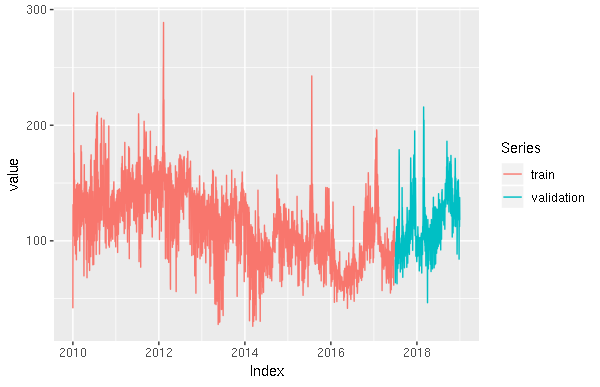
\includegraphics[width=\linewidth, height=7cm]{imgs/Series.png}
  \caption{Grafico della Serie}
  \label{fig:series}
\end{figure}\\
Dal dataset l'ultimo anno viene tenuto separato (Figura \ref{fig:series}), esso fungerà da test set sul quale verranno confrontati le varie metodologie di previsione.
Come metrica è stata scelta MAPE perché più capibile da un punto di vista umano, si poteva benissimo scegliere MSE o MAE.
Mentre per il confronto nelle metodologie stesse, i.e., diversi iperparametri o architetture si sceglieranno delle metriche diverse, e verranno dette quando si spiega ciascun modello.

\section*{ARIMA}
Si usa la classe xts per definire la serie temporale (xts perché la serie è giornaliera nei vari anni), plottando ACF e PACF (Figura \ref{fig:ACF_1}) si vede immediatamente l'esistenza di tutte tre componenti stagionali con stagionalità 7: AR$(1)_7$I$(1)_7$MA$(1)_7$ poiché si vede una discesa geometrica (ogni 7 giorni) nel grafico della PACF e una discesa lineare (ogni 8 giorni) nel grafico della ACF, l'esistenza della parte di integrazione stagionale si può vedere anche facendo un modello SARMA$(1,1)_7$ e vedendo che il coefficiente di SAR risulta essere molto vicino ad 1. 
\begin{figure}[!h]
  \centering
  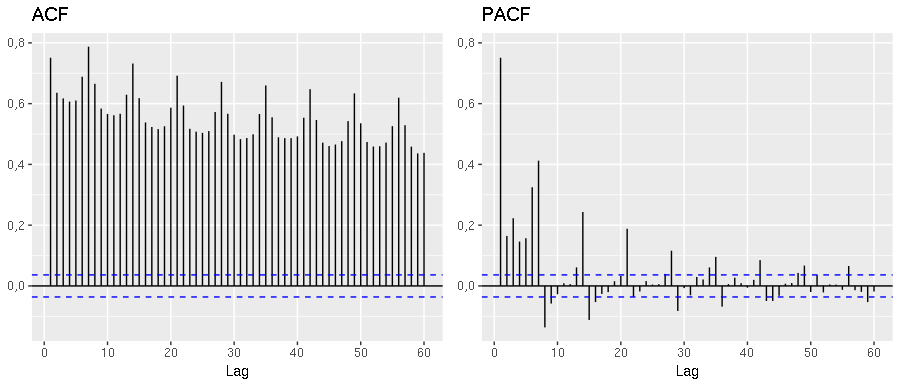
\includegraphics[width=\linewidth,height=5cm]{imgs/ACF_1.png}
  \caption{ACF e PACF della Serie.}
  \label{fig:ACF_1}
\end{figure}\\
Vi sembra essere anche quale componente non stagionale oltre ad una possibile parte di integrazione dovuta all'esistenza di qualche trend nella serie, ciò viene studiato sui residui dopo aver applicato il modello SARIMA$(1,1,1)_7$.
Sui grafici della ACF/PACF dei residui (Figura \ref{fig:ACF_2}) si vede che c'è un modello ARMA ma non si riesce a capire facilmente quali siano i coefficienti.
Per questa ragione si effettua una Grid Search con i coefficienti (potenze del polinomio caratteristico) di AR e MA che variano da 0 a 6, e scegliamo il modello con la log-likelihood più alta: Il modello con la log-likelihood più alta risulta essere un ARMA(6,6), ma plottando le radici e calcolandone i moduli vediamo che sono molto vicini ad 1, ciò significa che la serie aveva, come già si sospettava,  una parte di integrazione, si prova con la prima integrazione e questo problema viene risolto, quindi il modello finale proposto è un ARIMA$(6,1,6)(1,1,1)_7$.\\
\begin{figure}[!h]
  \centering
  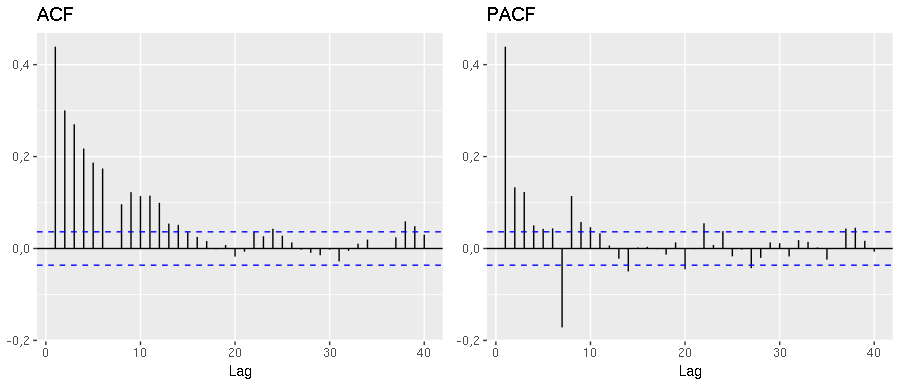
\includegraphics[width=\linewidth,height=5cm]{imgs/ACF_2.png}
  \caption{ACF e PACF dei residui del primo modello.}
  \label{fig:ACF_2}
\end{figure}
\begin{figure}[!h]
  \centering
  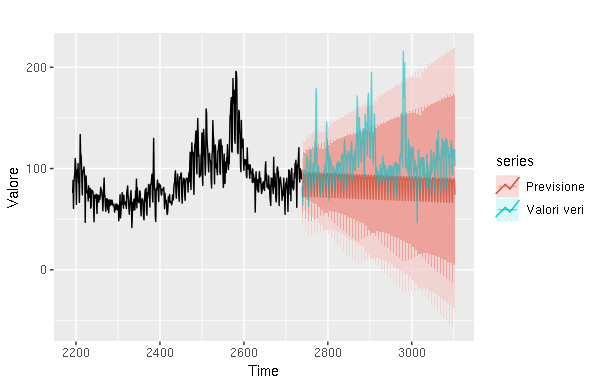
\includegraphics[width=\linewidth,height=6cm]{imgs/forecast_ar_1.png}
  \caption{Previsione della Serie sul Validation.}
  \label{fig:ARIMA_pred}
\end{figure}\\
Dalle previsioni di questo modello, mostrate nella Figura \ref{fig:ARIMA_pred}, si capisce immediatamente che queste componenti non spiegano tutta la varianza del modello, infatti questa serie è una serie multi stagionale, R non permette di trattare ARIMA multi stagionale quindi si introducono dei regressori esterni.\\
Per risolvere il problema di multi stagionalità si usano 24 regressori sinusoidali con frequenza base annua, il numero 24 è stato calcolato usando il validation set.
Si aggiungono altri regressori esterni: i giorni festivi, dando più importanza alle festività più importanti come il natale, pasqua, ferragosto e il nuovo anno e raggruppando le altre festività in un'unica variabile.
\begin{figure}[!h]
  \centering
  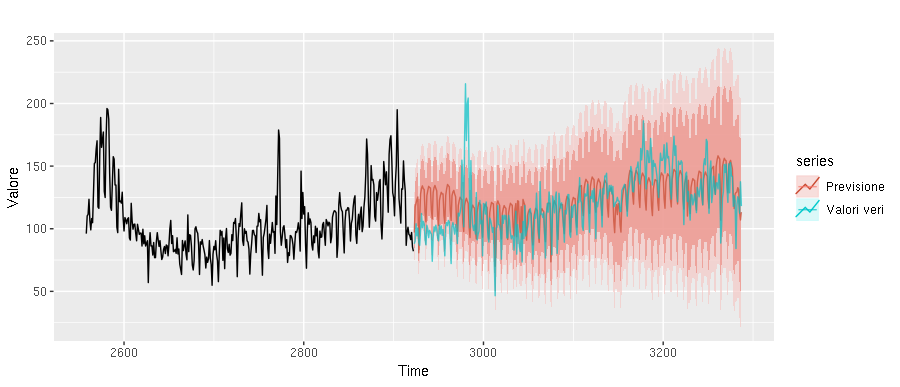
\includegraphics[width=\linewidth,height=6cm]{imgs/forecast_ar_2.png}
  \caption{Previsione sul Validation usando regressori.}
  \label{fig:XARIMA_pred}
\end{figure}\\
Nella figura \ref{fig:XARIMA_pred} si vede subito che questi regressori spiegano molta varianza del modello.

\section*{UCM}



\end{document}